\section{Automaten}

\begin{frame}{Endliche Automaten}
	Ein deterministischer endlicher Automat...
	\begin{itemize}
		\item ... besteht aus endlich vielen Zuständen
		\item ... ist zu jedem Zeitpunkt in \emph{genau einem} dieser Zustände
		\item ... wechselt bei Eingabe \emph{genau eines} Zeichens den Zustand in \emph{genau einen, definierten} Folgezustand
		\item ... und gibt dabei ein Wort als Ausgabe aus
	\end{itemize}

	Die gültigen \enquote{Zustandswechsel} sind als Zustandsübergänge definiert.
\end{frame}

\begin{frame}{Anwendungen}
	\begin{itemize}
		\item Getränkeautomaten
		\item Textsuche
		\item Textersetzung
	\end{itemize}

	Für Beispiele zur Textsuche und Textersetzung: Übung~12, WS~15/16
\end{frame}

\subsection{Mealy-Automaten}
\begin{frame}{Mealy-Automat}
	Bei einem Mealy-Automaten findet die Ausgabe \textbf{bei den Zustandsübergängen} statt.
	\begin{Definition}
		Ein Mealy-Automat $ A = (Z,z_0,X,f,Y,g)$ besteht aus $\dots$
		\begin{itemize}[<+->]
			\item $\dots$ einer endlichen Zustandsmenge $Z$ 
			\item $\dots$ einem Startzustand $z_0$.
			\item $\dots$ einem Eingabealphabet $X$ 
			\item $\dots$ einer Zustandsübergangsfunktion $f:Z\times X \to Z $
			\item $\dots$ einem Ausgabealphabet $Y$
			\item $\dots$ einer Ausgabefunktion $g:Z\times X \to Y^* $ 
		\end{itemize}						
	\end{Definition}
\end{frame}

\begin{frame}{}
	\begin{block}{Graphische Darstellung}
		Meistens werden kleine Automaten graphisch dargestellt. (Achtung: Die formale Schreibweise wird trotzdem auch im Studium verwendet! Also auswendig lernen!)\\
		Zustände sind Knoten und Übergänge gerichtete Kanten in einem Graphen!\\
		\textbf{Der Startzustand wird mit einem Pfeil \enquote{aus dem Nichts} gekennzeichnet!}\\ \pause
		\textbf{NICHT VERGESSEN!} Das kostet Punkte! Immer!
	\end{block}
\end{frame}

%% Übung: Beispiel
\setbeamercolor{background canvas}{bg=}

\includepdf[pages=3]{U12.pdf}

\begin{frame}{Eingabe eines Zeichens}
	Was ist die Zustandsübergangsfunktion $f$? \\ \pause
	Bei Eingabe eines Symbols $x\in X$ und des aktuellen Zustands $z\in Z$ gibt uns die Zustandsübergangsfunktion an, in welchen Zustand $z'$ der Automat dann sein wird. \pause \\
	Formell: $$ f(z,x) = z' $$ 
\end{frame}

\begin{frame}{Eingabe eines Wortes}
	Was machen wir mit ganzen Wörtern? \\ \pause
	Wir definieren uns ganz analog
	\begin{block}{Zustandsübergangsfunktion extended}
	\begin{align*}
		 	f_*(z,\varepsilon) &= z \\
		 	\forall w\in X^* \ \forall x\in X : f_*(z,wx) &= f(f_*(z,w),x) 
	\end{align*}
	\end{block}
	\pause Was macht diese Funktion? \\ \pause
	Bei Eingabe eines Wortes $w$ und Anfangszustand $z$ gibt sie den Zustand $z' = f_*(z,w)$ aus, in dem der Automat enden wird. 
\end{frame}
	
\begin{frame}{Eingabe eines Wortes}
	Definieren wir nun weiter 
	\begin{block}{Zustandsübergangsfunktion extended extended}
		\begin{eqnarray*}
			f_{**}(z, \eps) &=& z \\
			\text{und für alle $x\in X$ und $w\in X^*$ ist\ }
			f_{**}(z, xw)   &=& z \cdot f_{**}(f(z,x),w) \\
		\end{eqnarray*}
	\end{block}
	\pause Was macht diese Funktion? \\ \pause
	Diese Funktion gibt die Reihe aller Zustände aus, die der Automat bei Eingabe des Wortes $w$ im Startzustand $z$ durchläuft. 
\end{frame}

\begin{frame}{Eingabe eines Wortes}		
	Alternative Definition:
	\begin{block}{Zustandsübergangsfunktion extended extended}
		\begin{align*}
			f_{**}(z,\varepsilon) &= z \\
			\forall w \in X^* \ \forall x \in X : f_{**}(z,wx) &= f_{**}(z,w)\cdot f(f_*(z,w),x)	 
		\end{align*}
	\end{block}
\end{frame}

\begin{frame}{Beispiel: Ein Getränkeautomat}
	$R$ sei reines Wasser, $Z$ ist Zitronenlimonade, $O$ ist OK (Getränkeausgabe), $C$ ist Clear und $1$ ist die Eingabe von einer Münze mit Wertigkeit 1\\
	Wir wollen: \pause
	\begin{itemize}[<+->]
	 	\item Getränk wählen können
	 	\item Geld rein- und rausholen können
	 	\item und immer zurück kommen können!
	\end{itemize}
\end{frame}

\begin{frame}
	\begin{figure}[H]
		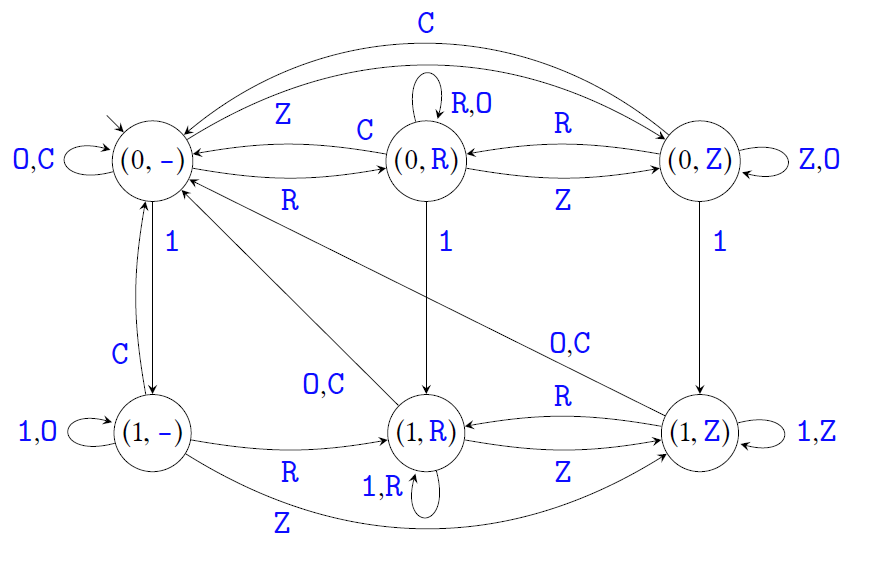
\includegraphics[scale=0.4]{automaten/getraenkeOhneAusgabe}
	\end{figure}

	Was macht $f((0,-), Z), f_*((0,-),R10) , f_{**}( (0,-),R10) $ ? Rechnerisch und graphisch.	

\end{frame}

\begin{frame}
	Rechnerisch nur der 3. Fall:
	\begin{align*}
		f_{**}((0,-),R10) =& f_{**}((0,-),R1) )\cdot f(f_*((0,-),R1),0) \\ 
		=& f_{**} ((0,-),R) \cdot f(f_*((0,-),R),1) \\ &\cdot f(f_*((0,-),R1),0) \\ 
	=& f_{**}((0,-),\varepsilon) \cdot f(f_*((0,-),\varepsilon),R) \\ &\cdot f(f_*((0,-),R),1) \cdot f(f_*((0,-),R1),0) \\ 
	=& (0,-) \cdot f((0,-),R) \cdot f( f(f_*((0,-),\varepsilon),R),1) \\ &\cdot f( f(f_*((0,-),R),1),0) \\
	=& (0,-) \cdot f((0,-),R) \cdot f( f((0,-),R),1)  \\ &\cdot f(f(  f(f_*(0,-),\varepsilon),R), 1), 0) \\
	=& (0,-) \cdot f((0,-),R) \cdot f( f((0,-),R),1)\\ &  \cdot f( f(f((0,-),R),1),0) \\ 
	= & (0,-) \cdot (0,R) \cdot (1,R) \cdot (0,-) 
	\end{align*} 
\end{frame}

\begin{frame}{Ausgaben}
	Nun betrachten wir einen Automaten mit Ausgabemöglichkeit. Die Kanten sind nun beschriftet mit $x \mid y$ , wobei $x\in X, y\in Y^* $. Also wird bei Eingabe von $x$ das Wort $y$ ausgegeben. \\ 
	Formal: $$g(z,x) = y$$
\end{frame}

\begin{frame}
	\begin{block}{Ausgabefunktion extended}
		Wir können also analog zu $f_*$ und $f_{**}$ definieren
		\begin{align*}
		g_* : Z\times X^* &\to Y^* \\
		g_*(z,\varepsilon) &= \varepsilon \\
		\forall w\in X^* \; \forall x\in X : g_*(z,wx) &= g(f_*(z,w),x) \\ \\
		g_{**} : Z\times X^* &\to Y^* \\ 
		g_{**}(z,\varepsilon) &= \varepsilon \\
		\forall w\in X^* \; \forall x\in X : g_{**}(z,wx) &= g_{**}(z,w)\cdot g_*(z,wx) 			
		\end{align*} \pause
	\end{block}
	
	Dies gibt nun nicht die durchlaufenen Zustände bzw. den Abschlusszustand an, sondern die letzte Ausgabe bzw. alle durchlaufenen Ausgaben. 

\end{frame}

\begin{frame}{Beispiel}
	\begin{figure}[H]
		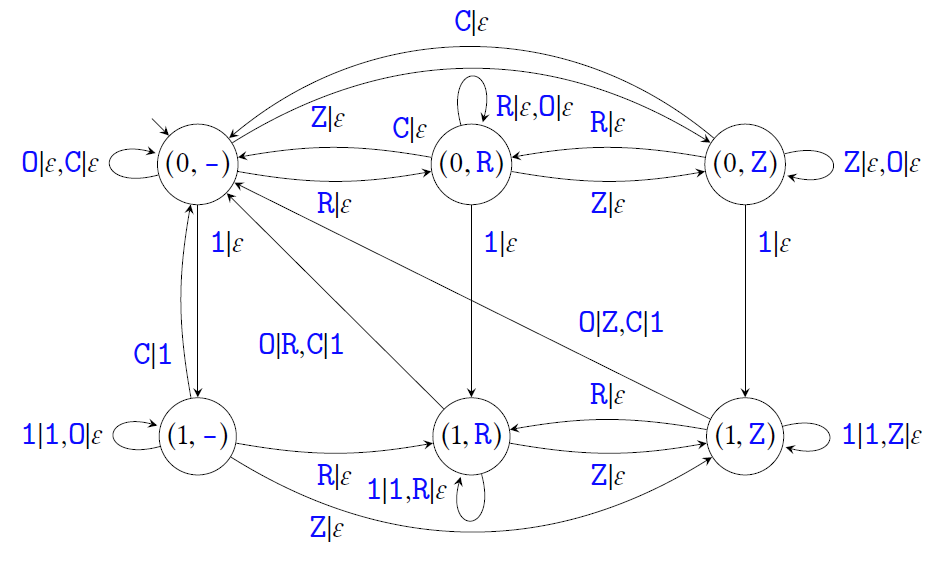
\includegraphics[scale=0.4]{automaten/getraenke}			
	\end{figure}
	Was macht $g_*((0,-),R10) , g_{**}((0,-),R10) , g_{**}((0,-),R110) $ ? \\ \pause
	$g_*((0,-),R10) = g_{**}((0,-),R10) = R, \qquad g_{**}((0,-),R110) = 1R $	
\end{frame}
	

\subsection{Moore-Automat}
\begin{frame}{Moore-Automat}
	Moore-Automaten sind ähnlich aufgebaut wie Mealy-Automaten.\\
	Unterschied: Ausgabe erfolgt im Zustand, nicht beim Zustandsübergang. \\ \pause 
	
	Ausgabefunktion: $h:Z\to Y$\\
	Dann ist $$ g_* (z,w) = h(f_*(z,w)) $$
	\pause
	Für $g_{**}$ gilt dann mit $h^{**}:Z^*\to Y$  $$ g_{**}(z,w) = h^{**} (f_{**}(z,w)) $$
	Wir wenden also $h$ auf jeden durchlaufenen Zustand an.
\end{frame}

% TODO
\begin{frame}{}
\end{frame}

%% Übung: Beispiel
\setbeamercolor{background canvas}{bg=}

\includepdf[pages=11]{U12.pdf}

\begin{frame}{}
	\begin{block}{Von Moore zu Mealy}
		Relativ straightforward.\\
		Ausgaben \enquote{aus den Knoten auf die Übergänge ziehen}\\
		Beachte: Für die Eingabe $\eps$ kann ein Moore-Automat eine Ausgabe $g_{**}(s, \eps) = \neq \eps$ erzeugen, ein Mealy-Automat \emph{jedoch nicht}.
	\end{block}

	\begin{block}{Von Mealy zu Moore}
		Komplizierter
	\end{block}
\end{frame}

%% Übung: Beispiel
\setbeamercolor{background canvas}{bg=}

\includepdf[pages={34-40}]{U12.pdf}

